\chapter{Labeling Problems - Graceful Numbering}

Rishnak found Ajur and Jura walking near the water fountain. Rishnak continued the conversation about graphs. Rishnak said vertex coloring and edge coloring are kinds of labeling with the constraints that adjacent vertices and edges are not colored the same. There could be a lot of other labeling possible. Rishnak said that there is one interesting labeling called graceful numbering. Graceful numbering of a graph is to assign distinct numbers to vertices  from $0, 1,2, \cdots, e$ such that all the edge labels/numbers are from distinct from $1,2, \cdots, e$. ($n$ is the number of vertices and $e$ is the number of edges). Rishnak added that the edge number is the absolute difference between the numbers associated with end vertices.
Rishnak illustrated with an example of a star tree ( A center vertex is connected to leaf vertices) see Figure \ref{19g1}

\begin{figure}
\begin{center}
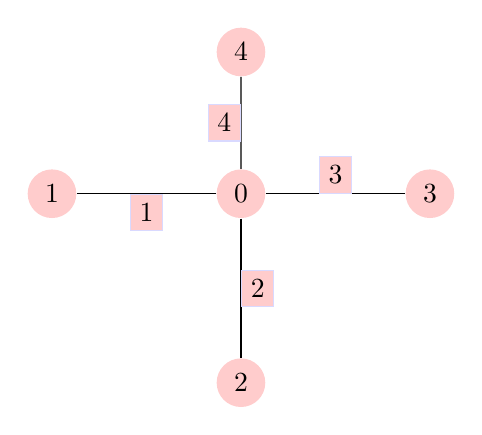
\begin{tikzpicture}
  [scale=.6,auto=left,every node/.style={circle,fill=red!20}]
  \tikzstyle{weight} = [draw=blue!15,shape=rectangle]
  \node (n1) at (5,5) {0};
  \node (n2) at (1,5)  {1};
  \node (n3) at (5,1)  {2};
  \node (n4) at (9,5) {3};
  \node (n5) at (5,8)  {4};
\foreach \source /\dest /\weight in {n1/n2/1,n1/n3/2,n1/n4/3,n1/n5/4} 
   \draw (\source) --node[weight] {$\weight$}  (\dest);


\end{tikzpicture}
\caption{A star tree gracefully labeled. All the edges get distinct numbers (difference between the labels of end vertices}\label{19g1}
\end{center}
\end{figure}
Ajur tried to do this for a simple path (some times called snake). He was able to gracefully label the path of length 5 Figure \ref{19g2}. Like Star tree, this snake can also be generalized to arbitrary number of vertices.

\begin{figure}
\begin{center}
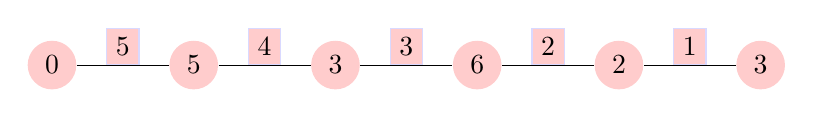
\begin{tikzpicture}
  [scale=.6,auto=left,every node/.style={circle,fill=red!20}]
  \tikzstyle{weight} = [draw=blue!15,shape=rectangle]
  \node (n1) at (1,1) {0};
  \node (n2) at (4,1)  {5};
  \node (n3) at (7,1)  {3};
  \node (n4) at (10,1) {6};
  \node (n5) at (13,1)  {2};
  \node (n6) at (16,1) {3};
\foreach \source /\dest /\weight in {n1/n2/5,n2/n3/4,n3/n4/3,n4/n5/2,n5/n6/1} 
   \draw (\source) --node[weight] {$\weight$}  (\dest);


\end{tikzpicture}
\caption{A path(snake) gracefully labeled. All the edges get distinct numbers (difference between the labels of end vertices}\label{19g2}
\end{center}
\end{figure}

For a binary tree with 7 vertices, Ajur could find a graceful numbering see Figure \ref{19g3}

\begin{figure}
\begin{center}

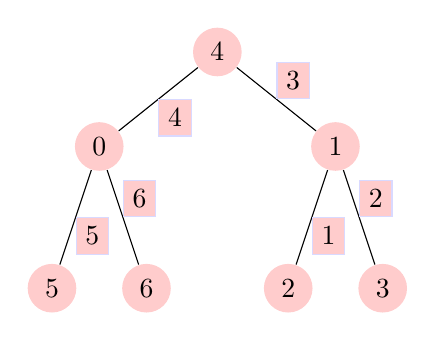
\begin{tikzpicture}
  [scale=.6,auto=left,every node/.style={circle,fill=red!20}]
  \tikzstyle{weight} = [draw=blue!15,shape=rectangle]
  \node (n1) at (5.5,7) {4};
  \node (n2) at (3,5)  {0};
  \node (n3) at (8,5)  {1};
  \node (n4) at (2,2) {5};
  \node (n5) at (4,2)  {6};
  \node (n6) at (7,2)  {2};
  \node (n7) at (9,2)  {3};
\foreach \source /\dest /\weight in {n1/n2/4,n1/n3/3,n2/n4/5,n2/n5/6,n3/n6/1,n3/n7/2} 
   \draw (\source) --node[weight] {$\weight$}  (\dest);
  
\end{tikzpicture}

\caption{A Binary tree with 7 vertices gracefully numbered }\label{19g3}
\end{center}
\end{figure}

One of the open questions (That means no one has solved) to show whether all trees admit a graceful numbering. It is not even known whether all binary trees admit a graceful numbering. They have
  tried to find counterexamples (some trees do not have graceful numbering) and failed. Their proof efforts to show all trees have a graceful numbering also did not succeed.
  
  There are graphs which do not have a graceful numbering like a cycle of length 5. Figure \ref{19g4}

\begin{figure}
\begin{center}

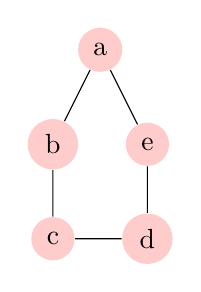
\begin{tikzpicture}
  [scale=.6,auto=left,every node/.style={circle,fill=red!20}]

  \node (n1) at (4,1) {a};
  \node (n2) at (3,-1)  {b};
  \node (n3) at (3,-3)  {c};
  \node (n4) at (5,-3) {d};
  \node (n5) at (5,-1)  {e};
 
\foreach \from/\to in {n1/n2,n2/n3,n3/n4,n4/n5,n5/n1}
    \draw (\from) -- (\to);
  
\end{tikzpicture}

\caption{Cycle of length 5 $C_5$ cannot be gracefully labeled }\label{19g4}
\end{center}
\end{figure}

A complete bi-partite graph $K_{m,m}$ can be gracefully colored/numbered by numbering vertices in one partition from $0,1,\cdots,m-1$ and the vertices
in the other partition from $m,2m,3m,\cdots m^2$. With this numbering all the edges get distinict numbers. Rishnak gave an example for this when $m=3$ - See Figure \ref{18g45}

\begin{figure}
\begin{center}

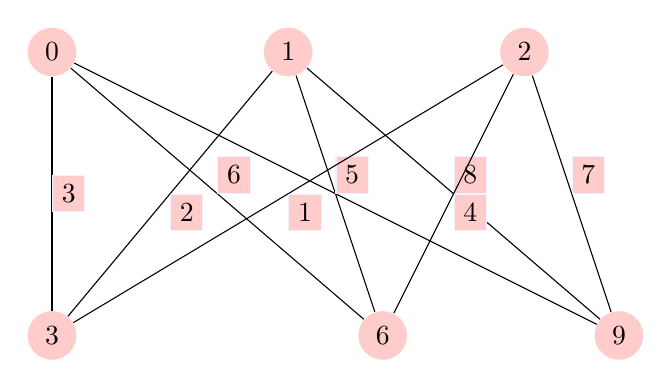
\begin{tikzpicture}
  [scale=.6,auto=left,every node/.style={circle,fill=red!20}]
  \tikzstyle{weight} = [draw=blue!5,shape=rectangle]
  \node (n1) at (-1,5) {0};
  \node (n2) at (4,5)  {1};
  \node (n3) at (9,5)  {2};
  \node (n4) at (-1,-1) {3};
  \node (n5) at (6, -1) {6};
  \node (n6) at (11,-1)  {9};
 
\foreach \source /\dest /\weight in {n1/n4/3,n1/n5/6,n1/n6/9} 
   \draw (\source) --node[weight] {$\weight$}  (\dest);
\foreach \source /\dest /\weight in {n2/n4/2,n2/n5/5,n2/n6/8} 
   \draw (\source) --node[weight] {$\weight$}  (\dest);
\foreach \source /\dest /\weight in {n3/n4/1,n3/n5/4,n3/n6/7} 
   \draw (\source) --node[weight] {$\weight$}  (\dest);

 
  \end{tikzpicture}
\caption{Gracefully labeled $K_{3,3}$}\label{18g45}
\end{center}
\end{figure}
Rishnak said a Golomb ruler is closely related to graceful numbering.  A Golomb ruler is a set of marks at integer positions along an imaginary ruler such that no two pairs of marks are the same distance apart. The number of marks on the ruler is its order, and the largest distance between two of its marks is its length.
Golomb ruler of order 3 is $\{0,1,3\}$. Golomb ruler of order 4 is $\{0,1,4,6\}$ measures all numbers upto 6. Golomb ruler has applications in coding theory. Golomb ruler can be used to graceful label a complete graph on 4 vertices - see Figure \ref{19g5}
\begin{figure}
\begin{center}

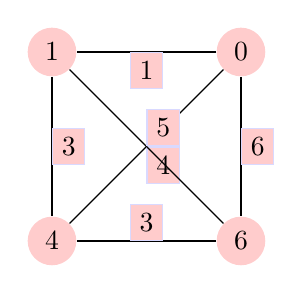
\begin{tikzpicture}
  [scale=.6,auto=left,every node/.style={circle,fill=red!20}]
  \tikzstyle{weight} = [draw=blue!15,shape=rectangle]
  \node (n1) at (5, -1) {0};
  \node (n2) at (1,-1)  {1};
  \node (n3) at (1,-5)  {4};
  \node (n4) at (5,-5) {6};

 \foreach \source /\dest /\weight in {n1/n2/1,n1/n3/4,n1/n4/6,n2/n3/3,n2/n4/5,n3/n4/3} 
   \draw (\source) --node[weight] {$\weight$}  (\dest);

  
\end{tikzpicture}

\caption{Complete Graph on 4 vertices $K_4$ gracefully labelled using Golomb Ruler}\label{19g5}
\end{center}
\end{figure}

Rishnak asked Ajur a puzzle from his favorite author Dudney (problem 453):
\textbf{In the present case a man has a yardstick from which 3 inches have
been broken off, so that it is only 33 inches in length. Some of the graduation
marks are also obliterated, so that only eight of these marks are legible; yet
he is able to measure any given number of inches from 1 inch up to 33 inches.
Where are these marks placed? }.

Ajur realized that this problem is similar to Golomb Ruler. 

Ajur started with earnest and he did not realize that one hour passed away so quickly. Ajur gave 11 solutions to this problems and added there are more than 50 solutions! Ajur's solutions where the 8 markings are in 33' ruler are as follows.
\begin{itemize}
    \item 1, 2, 3, 4, 10, 16, 22, 28
    \item 1, 2, 3, 4, 10, 17, 22,  28
    \item 1, 2, 3, 8, 14, 20, 24, 29
    \item 1, 2, 3, 10, 15, 22, 27, 31
    \item 1, 2, 3, 10, 16, 21, 25, 29
     \item 1, 2, 3, 11, 17, 21, 26, 30
     \item 1, 2, 3, 14, 18, 23, 25, 29
     \item 1, 2, 3, 14, 18, 23, 26, 29
     \item 1, 2, 3, 16, 21, 22, 26, 30
     \item 1, 2, 3, 16, 21, 24, 27, 31
     \item 1, 2, 4, 11, 18, 25, 30, 31
\end{itemize}
Rishnak  realized that Ajur had used a systematic brute force technique to solve this problem. So he decided that he would talk about Search Techniques the next day.
Ajur was so happy to learn a new type of ruler - that too an efficient ruler and how is it connected to Graceful numbering. Both of them felt happy and they called it a day.